

%\begin{figure}[t]
%\centering 
%\includegraphics[width=\linewidth]{figures/cutting-eq.eps}
%\caption{\label{fig:cutting-eq}Visual mapping between stack bar intervals %and instances.}
%\end{figure}

%SENTENCES DUMP

%Our data comprise of a dense set of macromolecules, encapsulated in compartments with several degrees of nesting. 
%Molecules are grouped by type and compartment, this information is contained in the scene file generated by cellPACK.
%Basic filtering parameters allows to manipulate the visibility of entire set of instances based on their type, independently or not from a geometrical cull object.
%Each cull object has its own parameters which are defined for all the ingredients type as shown in the overview Figure XX.
%When associated with geometrical shape, the cull object will only be influence to the region defined by the geometry, e.g, plane, sphere, cone...
%The cut objects how instances shall be discarded and they are applied sequentially.
%Internally the filtering is applied just after the object-space culling as shown in figure XX.
%User can modify these filtering parameters via the user interface.
%Additionally, there are more parameters which can influence when an instance is culled and which are related to a geometrical shape, those are defined in section XX.
%Additionally to defining where instances will be clipped, our system offer the mean to selectively chose the concentration of displayed elements for each protein types.
%These values are controlled by the user via the user interface. 

%Prior to the rendering each single instance is evaluated to determine if it shall be rendered.
%The cut objects how instances shall be discarded and they are applied sequentially.
%Internally the filtering is applied just after the object-space culling as shown in figure XX.
%First is applied the filtering based the clip probability.
%For each instance, we compare a uniformly distributed random number with the clip probability.
%If the random number is higher than the probability, the instance is marked as culled, and will not be rendered. 
%The random number is initially set for each individual instance and remain the same, in order to guaranty reproducibility of the scene.
%Secondly, instances are filtered according to their biochemical properties, for each cut object and each protein types the user defines ranges values for the both quantities and molecular weight.
%Instances whose properties lie outside on these ranges are marked as culled and discarded.
%For the book-keeping is the clipped ingredient we count for each ingredient type how many instances where discarded in total, for all active cut object.

\begin{comment}  
\section{Clipping}
Clipping objects define which instances of a given ingredient type are displayed.
There are two ways of how a clipping object can influence the clipping: either in object-space or in view-space.

\subsection{Object Space Clipping}

\end{comment}  

\section{Object Space Clipping}

Clipping objects define how instances shall be discarded depending on their location or type.
They can operate either in object space or in view space.
In this Section, we will explain in detail how clipping objects operate in object space.

%There are two ways of how a clipping object can influence the clipping: either in object-space or in view-space.
%%%%%%%%%%%%%%%%%%%%%%
%Using an object-space approach, the clipping objects will discard instances independent of the viewing direction. 
%Clipping objects are applied consecutively as explained in Figure \ref{fig:o}. This operation is recomputed every frame.
%The first step of the process is to determine, for each instance, if they are located in the clipping region.
%Once the instances are localized, they will be clipped according to object-space clipping parameters, which we describe in Section \ref{ssec:clip_params}.
%Moreover, we introduce the distance field falloff, an advanced parametrization for generating customizable gradient clipping effects.

\subsection{Clipping Object Distance}
\label{localization}
%Although supported shapes have a rather simple topology, it may still be computationally expensive, using a mesh-based representation, to compute a signed distance for a large number of instances.
%Indeed, using a triangle-based discretization would imply computing the signed distance between the instances and every single triangle of the mesh.
%Using such representation instead reduces the problem of evaluating the signed distance to solving trivial equations.
%It is also possible to apply simple SDF operators to the distance field, such as translation, rotation and scaling.
%The clipping region can also be reversed by inverting the result of the signed distance function, offering users flexibility.
%For instance, using a spherical shape, the clip region would be set to the inside of the sphere by default, while in inverted mode it would correspond to the outside of the sphere. 
%Although the set of offered clipping shapes is yet limited, it would be trivial to enrich it using more complex SDF operators, such as union, to merge several shapes together in one single distance field, and thus obtain more complex clipping region shapes.
%The first task of the object-space clipping is to determine whether an instance is located in the clipping region.
%This operation is repeated every frame for each instance of the scene.
Clipping objects are associated with geometric shapes to specify a region of the domain that is influenced by the clipping.
Our system currently supports the following set of primitive shapes: plane, cube, sphere, cylinder and cone.
We compute the distance between the instance centroids and the clipping region to identify instances that lie inside that region.
To accelerate the computation, we solve the problem analytically using a mathematical description of the clipping region as a 3D signed distance field (SDF).

Due to the architecture of the rendering technique which is employed, the instances information (position, rotation, type, radius, etc.) is already stored on the GPU in large buffers using a structure of array layout.
To speed up the clipping operation and avoid data transfer costs, the distance is computed in parallel in a compute shader program, prior to the rendering, with one thread allocated per instance.  
The position, rotation, scale and geometry type of every clipping object must be additionally uploaded to the GPU in order to define the correct clipping region SDF.
In a single thread and for each clipping object, the required information is fetched from the video memory and is used to compute the signed distance between an instance and the clipping object.
When an object needs to be clipped, a dedicated flag in a GPU buffer is updated. The flag is read during the rendering to discard the clipped instance.

\subsection{Clipping Filtering} \label{ssec:clip_params}

A clipping object also comprises a set of parameters that override the clipping state of instances based on their type.
This filtering operation is performed if an instance is located inside the clipping region, in the same compute shader program described in Section \ref{localization}.
The first parameter controls the percentage of discarded instances in the clipping region for a given type.
We refer to this value as \emph{object space clipping probability}.
This value can be increased or decreased by dragging the light green bar in the visibility equalizer.
%Clipping objects are applied in serial, the output of a clipping object constitute the input of the next one. 
It is important to mention that with multiple clipping objects, interaction with the light green bar in the visibility equalizer will only affect the clipping probability of the selected clipping object.

Upon start-up of the system, each instance is given a uniformly distributed random number between $0$ and $1$, and which will remain unchanged.
Then, for each instance, we compare this value with the clipping probability in the computer shader program.
If the constant random number is higher than the clipping probability, the instance is marked as discarded, and will not be rendered. 
For example, if the clipping probability value is equal to zero, all instances in the clipping region will be clipped, whereas if the value is equal to one, no instances will be clipped.
A value between zero and one thus controls the degree of fuzziness of a clipping, as explained in Figure \ref{fig:falloff}.

The other parameters allow users to control the clipping based on properties such as the size of the molecules (weight) and their overall number (concentration).
Via the user interface and for a given clipping object, the user defines ranges that correspond to the desired concentration and molecular weight.
Instances whose properties lie outside these ranges are simply discarded and will not be rendered.

\subsection{Falloff Function}

\begin{figure}[t]
\centering
\subfloat[]{\label{fig:falloff0}\includegraphics[width=0.3\linewidth]{figures/__falloff0.eps}}
\subfloat[]{\label{fig:falloff1}\includegraphics[width=0.3\linewidth]{figures/__falloff1.eps}}
\subfloat[]{\label{fig:falloff2}\includegraphics[width=0.3\linewidth]{figures/__falloff2.eps}}
\caption{\label{fig:falloff} 
Illustration of the falloff function mechanism: (a) elements located further than distance $d$ from the clipping object  are clipped, (b) elements between the clipping object and $d$ are uniformly clipped, (c) elements are removed gradually based on their distance to the clipping object to further customize its behaviour.}
\vspace{-5mm}
\end{figure}


To increase control over the object space clipping, we use a falloff function. 
The falloff function gradually modulates the effect of the clipping with respect to the distance from the clipping shape as illustrated in Figure \ref{fig:falloff}.
%This is easily achievable, since we use distance functions to represent the clipping objects. 
%Therefore, the distance of a molecular instance from the clipping surface can be evaluated by simply sampling the distance function of the given clipping object at the 3D position of the instance. 
The farther away from the clipping surface an instance is, the higher its clipping probability will be.
%The falloff function can be either constant, linear, or exponential.
The object space clipping probability of a molecule on the 3D position $p$ is multiplied by the falloff function $f(p)$. The falloff function is defined as follows:
\begin{equation}
	f(\vec{p}) = 1 - min(1, (d(\vec{p}) / d) ^ c)
\end{equation}
where $d(p)$ is the distance to the clipping surface from the point $p$. 
The function is parametrized by $d$ and $c$, where $d$ is the maximum distance up to which the object space clipping probability takes effect, and $c$ specifies the exponent of the falloff function.
%We provide additional parameters to gradually remove instances according the shape of the clipping region. These parameters control the so-called \emph{falloff functions}
It is important to mention that the falloff function will not preserve the user-defined clip-ratio displayed in the visibility equalizer.
%An example of the falloff function applied to the object space clipping is shown in Figure \ref{fig:res:gh3}. 
%The molecules of the blood serum (shown in red) are gradually removed from the bottom to the top. 
%In this way, the information about the concentration of these molecules is illustrated at the bottom of the scene, while the visibility of the HIV particle (blue and green) is increased towards to top of the scene.
%\textbf{TODO PMINDEK:} Talk about gradient clipping here, motivation and parameters, maybe a figure too.

\section{View-Space Clipping}

While object space clipping with primitive shapes allows for a high degree of flexibility, it may also require cumbersome manual operations for more complex set-ups.
We therefore provide additional functionalities to selectively remove occluding instances in front of a set of ingredients set focus, to ensure them a maximum degree of visibility.
The focus state can be manually specified via the visibility equalizer by ticking a dedicated checkbox in front of the stack bars.
%We use occlusion queries to determine the instances located in front of the focus region. 
%We provide users with the option to control the degree of fuzziness of the clipping, similarly to object-space clipping.
%We also introduce a new effect inspired from the work of scientific illustrators, that allows users to control the degree of aperture of the view-space clipping.
%Finally, we modify our occlusion query method to improve depth perception. This is done by performing contextual anchoring which means that instances that would normally be clipped are kept when located in close vicinity to the focus region.

\subsection{Occlusion Queries}
\label{sec:OQ}
%Focus ingredients are priorly selected from the user interface.
%In order to clip instances that are occluding the focus region, the most optimum approach in terms of efficiency and ease of implementation is without a doubt image-based.
%Modern graphics hardware already a fixed function called occlusion queries (OQ) and which allow to determine whether an instance is visible or hidden according to previously drawn geometries.
%This approach, however, would require issuing one draw call per queries, which can seriously effect the frame rate when issuing hundred of thousands of queries, because of GPU driver overhead.
%The rendering tool we are using already allows to render the entire scene in a single call to avoid latency due to the GPU driver.
%Due to the potentially large number of instances in the scenes we showcase, we accelerate the computation of occluding instances using an image-based approach on the GPU.
%However, for the sake of simplicity, we decide to assign only one occlusion mask per clipping object.
%, however, only one mask texture can be generated per clipping object.
%To achieve zero GPU driver overhead, we perform custom occlusion queries in a single draw call, using the programmable graphics pipeline.
%Subsequently, we draw the bounding sphere of all remaining instances over the mask.
%Due to early depth-stencil test, implicitly performed by the graphics hardware, 

When an ingredient type is set as focus, occluding instances of a different type may be selectively removed to reveal the occludees.
To determine which are the occluding instances, we perform occlusion queries. 
Nowadays, modern graphics hardware is able to perform occlusion queries easily using the fixed-functionality.
However this method requires one draw call per query, which may induce driver overhead with several thousands of queries.
We compute the queries manually instead using a custom shader program, because it allows the queries to be computed in a single GPU draw call, thus approaching zero driver overhead.
In-depth technical details about this approach are described by Kubisch \& Tavenrath \cite{kubisch2014opengl}.

We first render all the focused ingredients to an off-screen texture. 
This texture will then serve as a depth-stencil mask for the occlusion queries.
There can be several ingredient types constituting the object of focus for a given clipping object.
Thereafter, we render the bounding spheres of the potential occluders in a single draw call using instancing, on top of the depth-stencil mask.
Thanks to early depth-stencil functionality, available on modern graphics hardware, fragments that will pass the test and be executed are guaranteed to belong to an occluder.
We then update the clipping state of the occluding instance by updating its corresponding occlusion flag stored in the main video memory directly from the fragment program.

%An example of how we perform occlusion queries is shown in Figure \ref{fig:df0}.

\begin{figure}[t]
\centering
\subfloat[]{\label{fig:df0}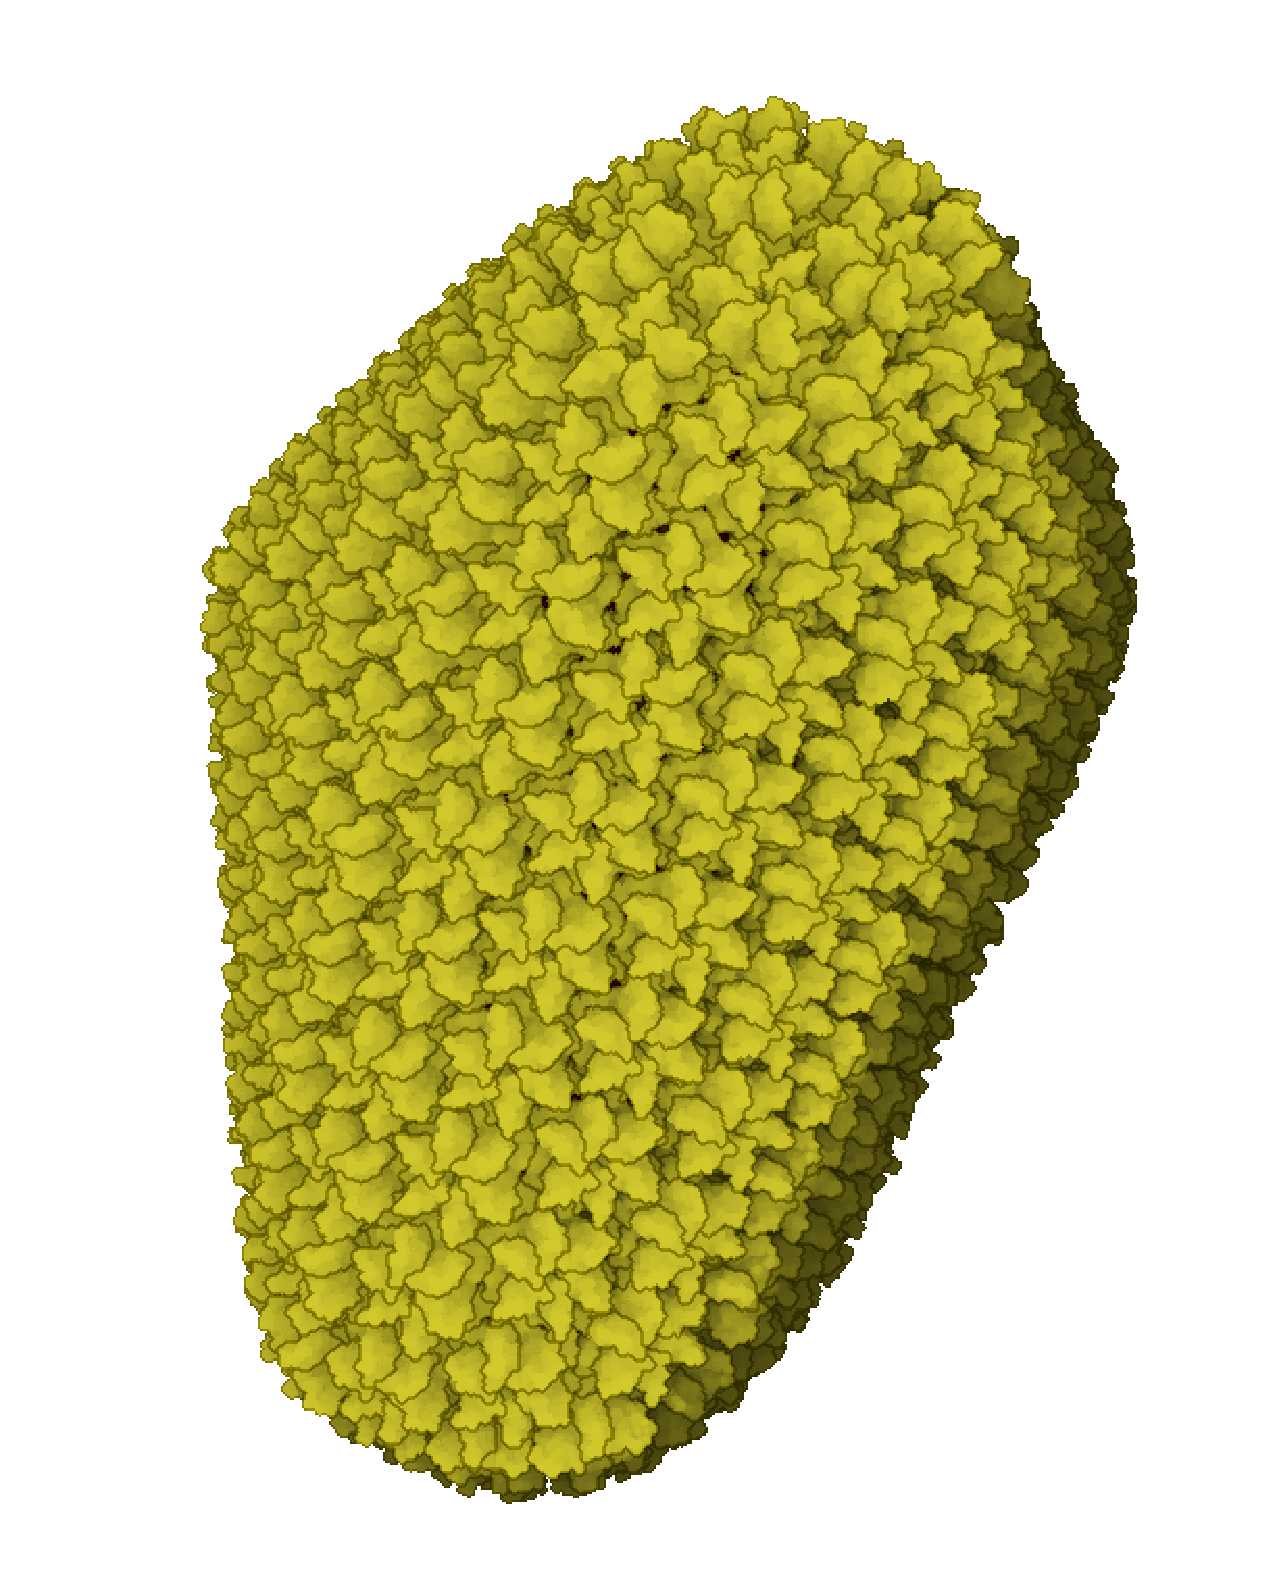
\includegraphics[width=0.25\linewidth]{figures/df0.eps}}
\subfloat[]{\label{fig:df1}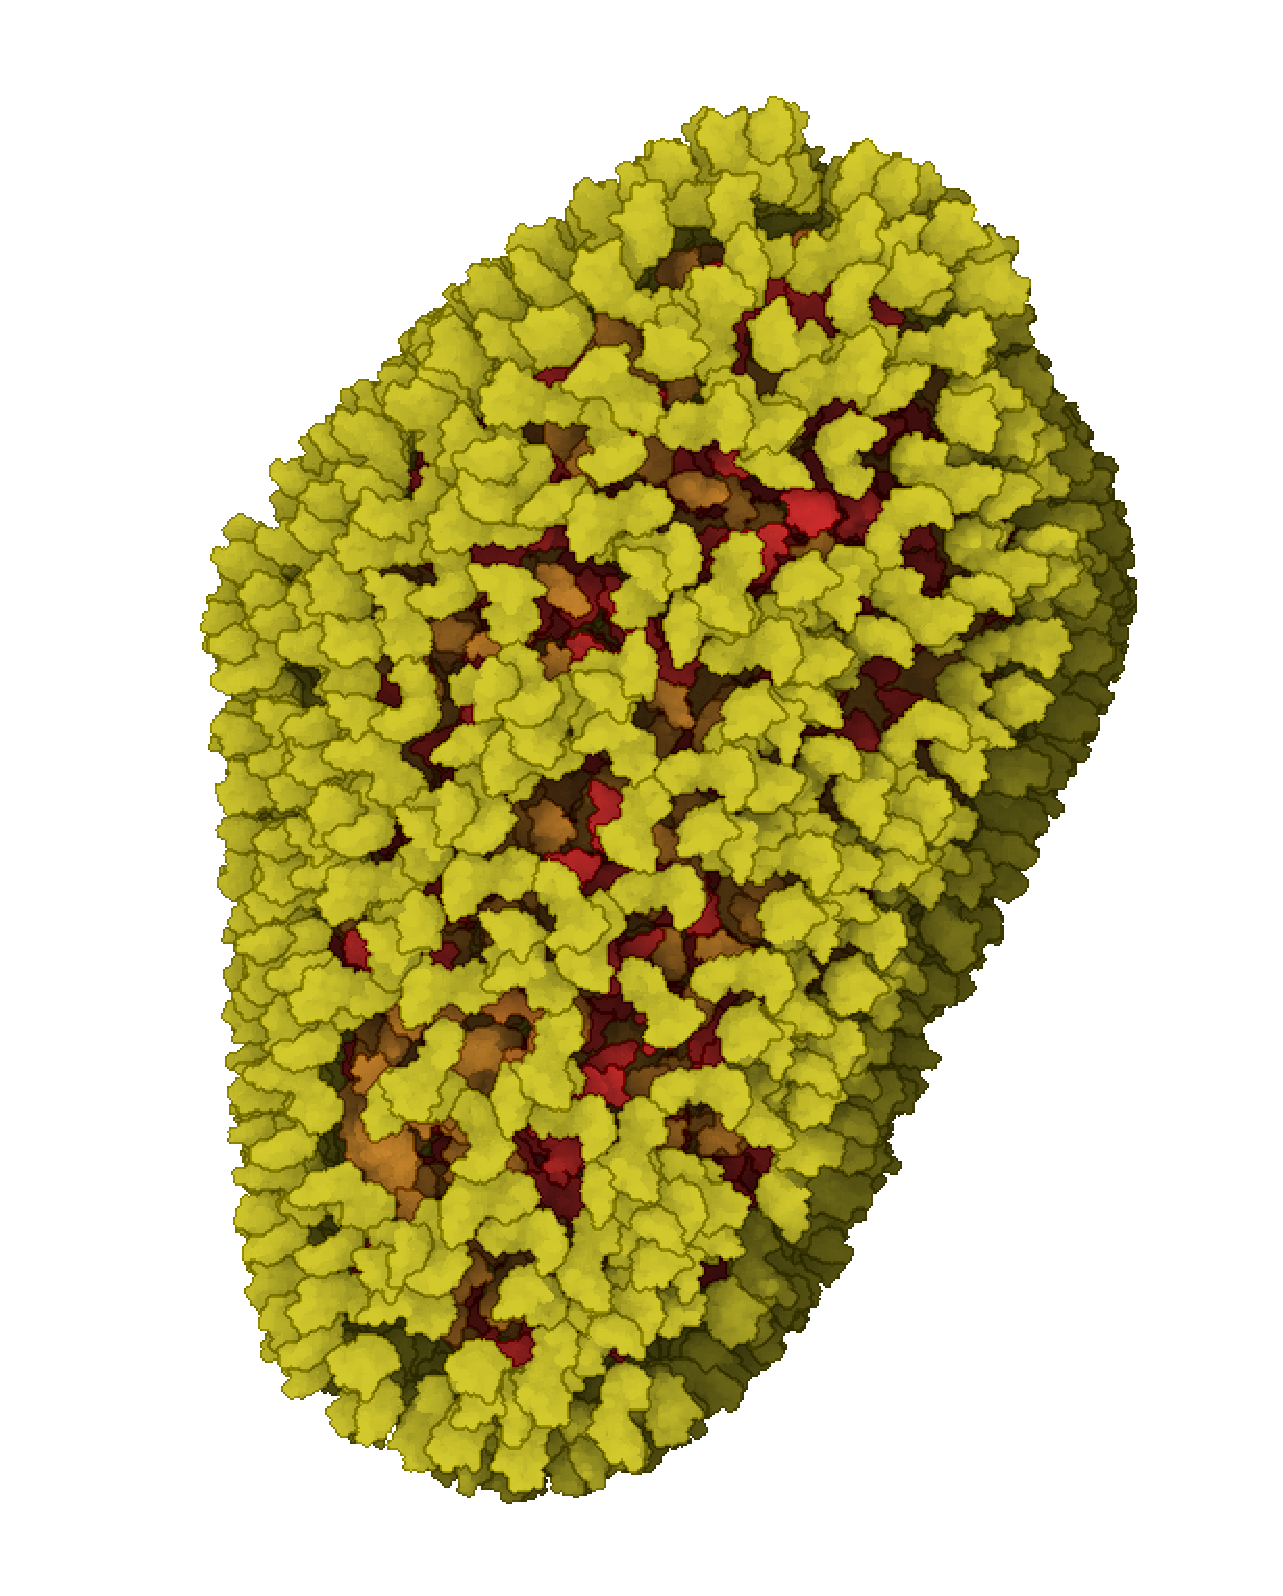
\includegraphics[width=0.25\linewidth]{figures/df1.eps}}
\subfloat[]{\label{fig:df2}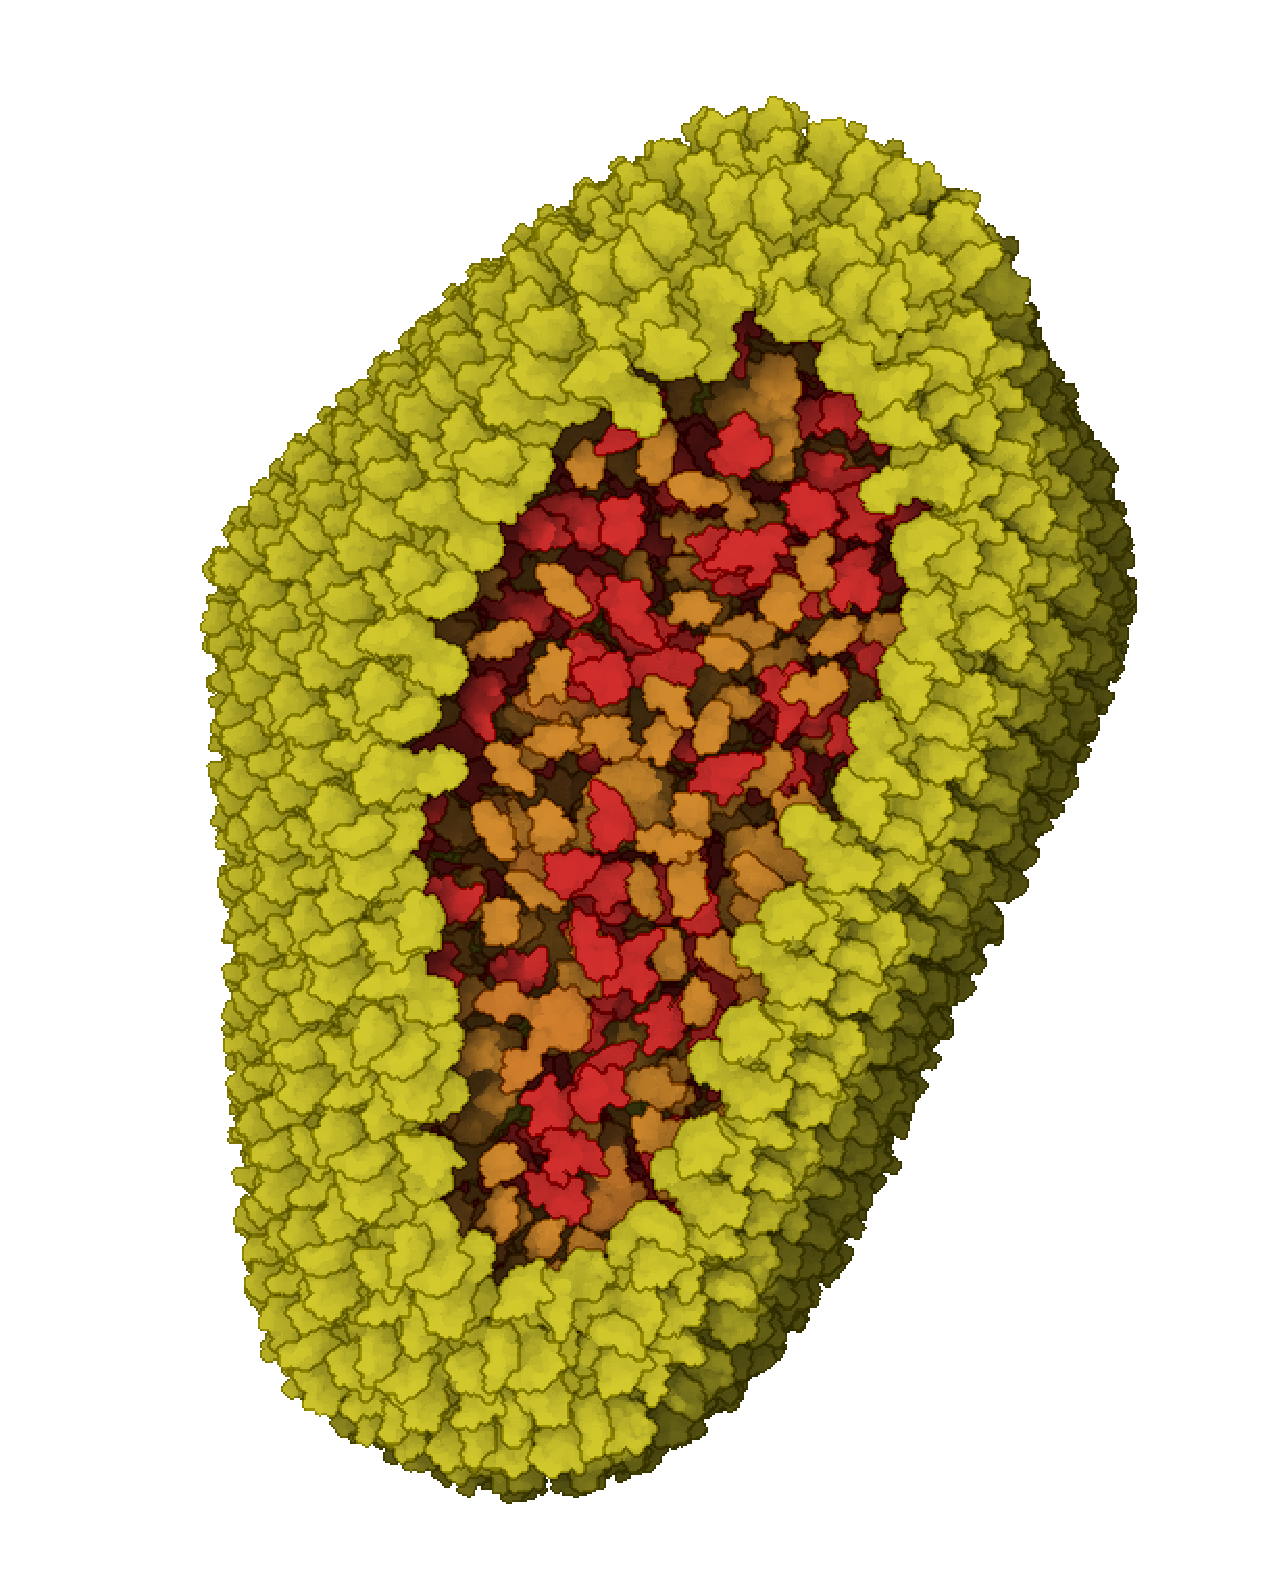
\includegraphics[width=0.25\linewidth]{figures/df2.eps}} 
\subfloat[]{\label{fig:df3}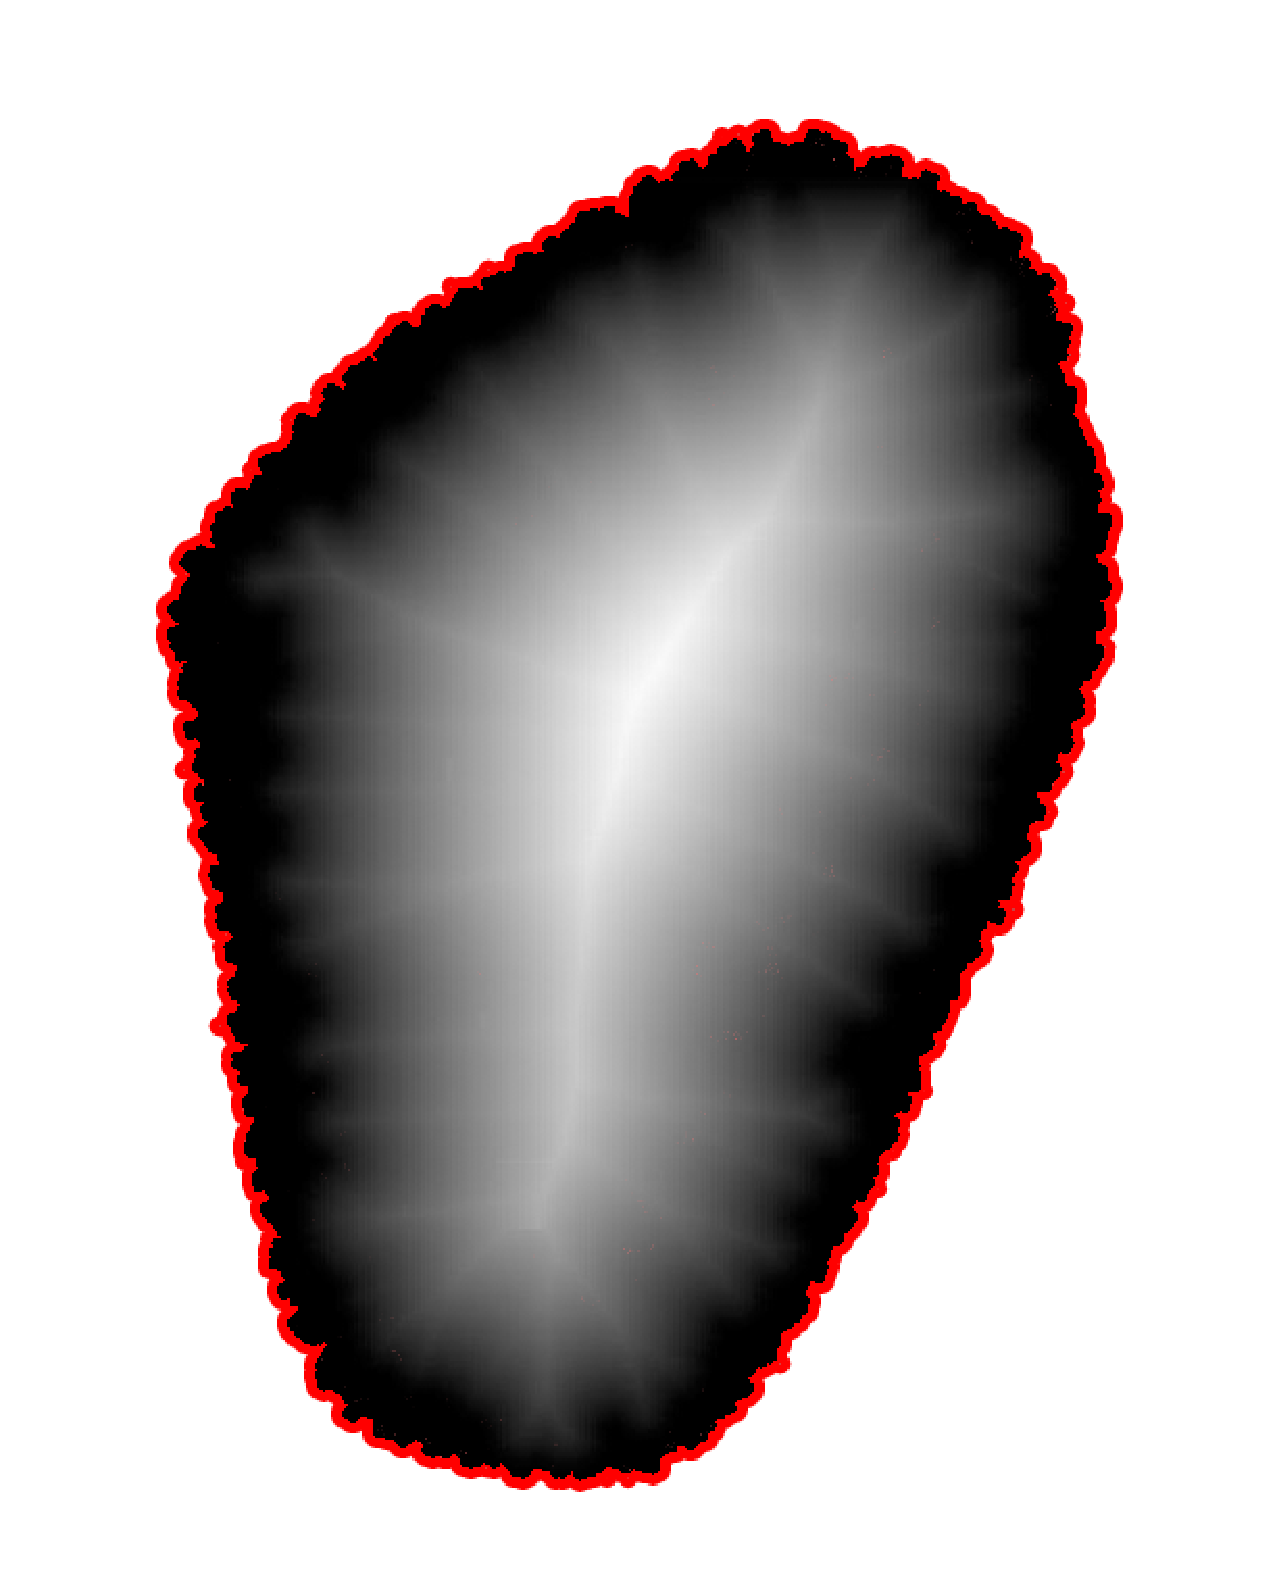
\includegraphics[width=0.25\linewidth]{figures/df3.eps}}
\caption{\label{fig:df}View-space clipping, (a) shows the full HIV Capsid, (b) shows the uniformly distributed clipping, (c) demonstrate the aperture effect and (d) shows the results of the 2D distance transform of the clipping mask.}
\vspace{-8mm}
\end{figure}

\subsection{Clipping Filtering}

Similarly to the object space clipping, we provide an additional parameter to control the degree of fuzziness of the view-dependent clipping, which we refer to as \emph{view-space clipping probability}.
This value is set by the user for each ingredient type, and is modified by dragging the dark green bar in the visibility equalizer.
The view-space clipping probability is evaluated after an instance was flagged as occluder in the same shader program mentioned in Section \ref{sec:OQ}.
We compare the clipping probability with a random number, initially defined and described in Section \ref{ssec:clip_params}.
If the random number is higher than the clipping probability, the instance will remain as clipped, otherwise it will be displayed. 
This will however result in a uniformly distributed number of visible occluders over the object of focus. 
Such a distribution might not always be the best design choice, because it fragments heavily the overall structure of the occluders and makes it difficult to see the occludees, as shown in Figure \ref{fig:df1}.

We propose an alternative technique for fuzzy removal of occluding instances, which we dub \emph{aperture effect}.
We define an additional parameter, the aperture coefficient, which controls the 2D distance from the instance to the edges of the occludees mask below which occluding instances shall be clipped.
A visual explanation of the aperture effect is shown in Figure \ref{fig:df2}.
To enable this effect we compute the 2D distance transform of the occludees mask which we store in a separate off-line texture.
We use the GPU Jump Flooding Algorithm by Rong \& Tan \cite{Rong06} to interactively recompute the 2D distance field every frame. 
After the computation of the distance transform, the texture stores the distance to the contours of the shape for each pixel.
Then, while computing occlusion queries in the fragment shader, we simply look-up the distance for the current fragment, and discard instances according to the user-defined aperture coefficient.
%, priorly set of each ingredient type.



\begin{figure}[t]
\centering
\includegraphics[width=0.7\linewidth]{figures/__hiv.eps}
\caption{\label{fig:hiv-islands} 
Illustration of contextual anchoring with an HIV particle. 
Despite the cutaway, some of the glyco-proteins (in yellow) are displayed and their surrounding lipid molecules (green) is preserved as contextual information.}
\vspace{-5mm}
\end{figure}

\subsection{Contextual Anchoring}
\label{ssec:anchoring}

When observing still images of cut-away scenes, it might be challenging to perceive the depth of objects correctly, despite using lighting-based depth cues.
We propose an additional method for depth guidance, which we call \emph{contextual anchoring}.
The concept is to override the results of clipping, to preserve elements located in proximity to non-clipped elements, and that would normally be clipped.
%By introducing contextual anchoring, the viewer, will intuitively understand where instances are located.
This principle in shown in Figure \ref{fig:hiv-islands}, where we can observe parts of the green membrane anchored around channel molecules, and which indicate that they are located on the surface of the object.
We were able to procedurally reproduce this effect by applying a depth bias to the occlusion queries computation for selected focused molecules.
This bias will ensure that contextual elements will no longer overlap the focus and will therefore be preserve as illustrated in Figure \ref{fig:islands}.



\begin{figure}[t]
\centering
\subfloat[]{\label{fig:df0}\includegraphics[width=0.45\linewidth]{figures/__islands-no.eps}}
\subfloat[]{\label{fig:islands1}\includegraphics[width=0.45\linewidth]{figures/__islands-yes.eps}}
\caption{\label{fig:islands} 
The principle of the depth-bias used for contextual anchoring.
The dark bars represents the depth values of the mask from the side, in one dimension. 
Elements in grey correspond to potentional occluders, while elements in red and green correspond to focused elements.
The red type is subject to contextual anchoring.
(a) Without contextual anchoring, the depth of occluders (grey) is overlapping the depth of the mask and will therefore be discarded. 
(b) With contextual anchoring, the depth of the occludees (red) is shifted so that context elements (purple) no longer overlap the focus and remain unclipped.}
\vspace{-3mm}
\end{figure}

\section{Equalizing Visibility}



%The first section of the histogram (dark green region) shows the percentage of instances that are currently visible on the screen. 
%The entire green section (dark \& light green) represents the percentage of instances that are actually rendered.
%To provide a clear overview of the scene properties, we display stack bars for each ingredient type that indicate information about their degree of visibility.

The visibility equalizer comprises a series of stack bars that convey important visibility information for each ingredient type.
The three colors correspond respectively to the number of visible, occluded and clipped instances, as explained in Figure \ref{fig:ohist}.
In order to fill the stacked bars with correct values, we must count the number of clipped and visible instances, and this operation must be repeated on every update.

\subsection{Counting Clipped Instances}

We perform the counting of the clipped instances on the GPU, in a dedicated compute shader program, since all the data already reside in the video memory.
We priorly declare a dedicated buffer on the GPU to hold the number of clipped instances for each ingredient type, and which shall be cleared before each counting operation.
Counting the clipped instances is a rather straightforward task since the clipping state of each instance is routinely computed and stored in a dedicated GPU buffer.
Once the clipping routine is performed, we simply browse through all the instances, and in case an instance was flagged as clipped, we increase the counter in the GPU buffer that corresponds to the number of clipped instances for the given type.
It is important to use an atomic increment operation for the counting to avoid concurrent accesses to the same counter value from different threads. 

\subsection{Counting Visible Instances}

In order to count the number of visible instances for a given view-point, we first need to generate an instance-buffer, which is a texture that contains, for each pixel, the unique instance id of the rendered molecule.
We first start to flag visible instances in a post-processing shader, by browsing all the pixels of the instance-buffer.
In case an instance is present in the instance-buffer, it is guaranteed to have at least one pixel visible on the screen, and it is therefore flagged as visible in a dedicated GPU buffer.
To store the number of visible instances per type, we also need to declare an additional GPU buffer, which must be priorly cleared each time visible instances are counted.
In a second stage, similarly to the counting of the clipped instances, we browse through all the instances in a dedicated compute shader, while fetching the visibility information which was previously computed.
Should an instance be flagged as visible, the counter that corresponds to the number of visible instances for the given type will be increase using an atomic increment operation.
Once the information about the number of visible and clipped instance is obtained, the data is then transferred to the CPU, and used to update the visibility equalizer.

\begin{comment}  

%\subsection{Visibility Tracking}

Modification of the visibility using the equalizer requires to know for each ingredient type, how many instances have been clipped and how many instances are actually visible on the screen, see Figure \ref{fig:ohist}.
Our system leverages the power of the GPU to compute the clipping state of each instance every frame.
Therefore, the information about clipping states is stored in the GPU memory.
In order to avoid an overhead due to data transfer between CPU and GPU, we perform the visibility tracking on the GPU using atomic operations.
%Atomic operations are parallel programming features which guarantee mutual exclusion when simultaneous thread wish to write in the same memory location.
We initially declare a buffer on the GPU to store the number of clipped and visible instances for each ingredient type.
To obtain the number of clipped instances, we simply increment the corresponding counter, each time an instance has been discarded using an atomic addition function.

For computing the number of visible instances, we first need information about actual visibility of rendered instances.
We render an additional off-screen texture where each pixel contains the internal ID of the instances.
We also declare an additional buffer to store a flag for each instance, which indicates if an instance is visible or hidden.
Then, by browsing through each pixel of the aforementioned ID texture in an additional pass, we update the visibility flag for the ID contained in each pixel.
Finally, we browse through each instance, and increment the corresponding counter according to the visibility flag using an atomic addition function, similar to the counting of clipped instances.

\subsection{User Interaction}

Upon interaction with the visibility equalizer, the system will either increase or decrease the number of clipped instances that correspond to the respective ingredient type.
This is intended to optimise the way users interact with the system, by offering a way to directly manipulate quantities rather than abstract internal values such as the clipping probability.
Additionally, the user may also manipulate more advanced parameters in an additional UI panel.
%We chose to map the motion of the histogram handles the clip probabilities.
%The first handle manipulates the view-space clipping probability, while the second handle controls the object-space one.
The clipping probabilities that are manipulated by the user correspond to the currently selected clipping object.
The displayed visibility in the equalizer, however, is valid for the entire scene.

%Quantities are relative by default, i.e, they represent a percentage of the total number of instances for a given ingredient.
%However, thanks to our design choices, they can also
Quantities shown in the visibility equalizer are ratios, not the absolute amounts. However, they can also be displayed as absolute quantities with limited additional effort.
For displaying absolute quantities, we support logarithmic scaling to ensure ingredients present in low quantities are visible in the stacked bars.
A logarithmic ruler is also provided to help the understanding of the displayed values.

\end{comment}  

%\section{Enhancements}

%Additionally to standard clipping functionality we developed a few enhancements to improve the way we perceive the scene.

%A crucial element when dealing with cluttered scenes is depth perception.

%Depth cues can be implemented by imitating the way light interact in reality to help us understanding distances between objects.

%However simulation illumination is rather expensive and prohibits a responsive user experience.

%We implement simplistic depth cues instead with a rough approximation of light behaviour.

%Additionally when provide option for context preserving view-space cut for a better understanding of the distance between objects in the view direction.

%Finally we perform rendering of the clipped element as ghosts in order to better communicate the overall proportions of visible elements in the scene.

%\subsection{Depth Cues}

%Depth cues are essential in molecular visualization and there exists many reference in the literature on how improve depth perception for that specific case.

%The first depth cue that we support is screen space ambient occlusion (SSAO) which allows to mimicate how global illumination works on the local scale, in image-space by evaluating for each pixel the depth of the surrounding pixels.

%Similarly to \cite{keylist}, we support two levels of ambient occlusion with different search radius to provide illumination for different levels of magnification.

%In addition to the limited range of the effect, SSAO does not account for directional light effects, which mean that shadows cannot be casted side-ways.

%When performing cut away however we perform strong shape alteration of the dataset which might be hard to perceive without shadows.

%Therefore, we additionally provide shadow mapping to better communicate the overall shape of the cuts.

%A downside of this approach is that it require an additional draw pass for each light that casts shadows onto molecules.

%Alternatively we also provide a cheaper method to provide additional cues about the shape of the clip objects.

%\textbf{TODO: PMINDEK, provide details about cheap depth cues}

%\subsection{Clipping Ghosts}

%While histograms allow us to visually monitor the quantities of removed instances, it might still be interesting to convey this information in the 3D scene while preserving  visibility settings.

%We additionally provide the option to render ghosts of all the clipped instances on top the scene, using alpha blending.

%We render all the ghosts in a separate off-screen texture which we later blend with the results of the scene rendering.

%The blending of the scene with the ghost texture is designed to ensure that the depth of the ghosts texture will merge with the scene's depth, and thus, that occluded ghosts will not be visible in the final results.

%We offer two rendering style for the ghosts, coloured filled or contour only.

%For each ingredient type we offer the option to render ghosts or not via the user interface.

%The resulting render of a scene with clipping ghosts can be seen in figure XX.
